\documentclass{article}
\usepackage[paperwidth=18cm,paperheight=7.5cm,margin=0cm,noheadfoot]{geometry}
\usepackage{amsmath,amssymb}
\usepackage{tikz}
\usetikzlibrary{arrows.meta,positioning,calc}
\usepackage{xcolor}
\pagestyle{empty}
\setlength{\parindent}{0pt}
\setlength{\parskip}{0pt}
\setlength{\topskip}{0pt}

% === Unified academic color palette ===
\definecolor{acadblue}{HTML}{2C5F8A}
\definecolor{acadpurple}{HTML}{7B4F9D}
\definecolor{acadorange}{HTML}{D4792A}
\definecolor{acadgreen}{HTML}{4CAF50}
\definecolor{acadred}{HTML}{E74C3C}
\definecolor{acadgray}{HTML}{95A5A6}

\begin{document}
\vspace*{0pt}\noindent
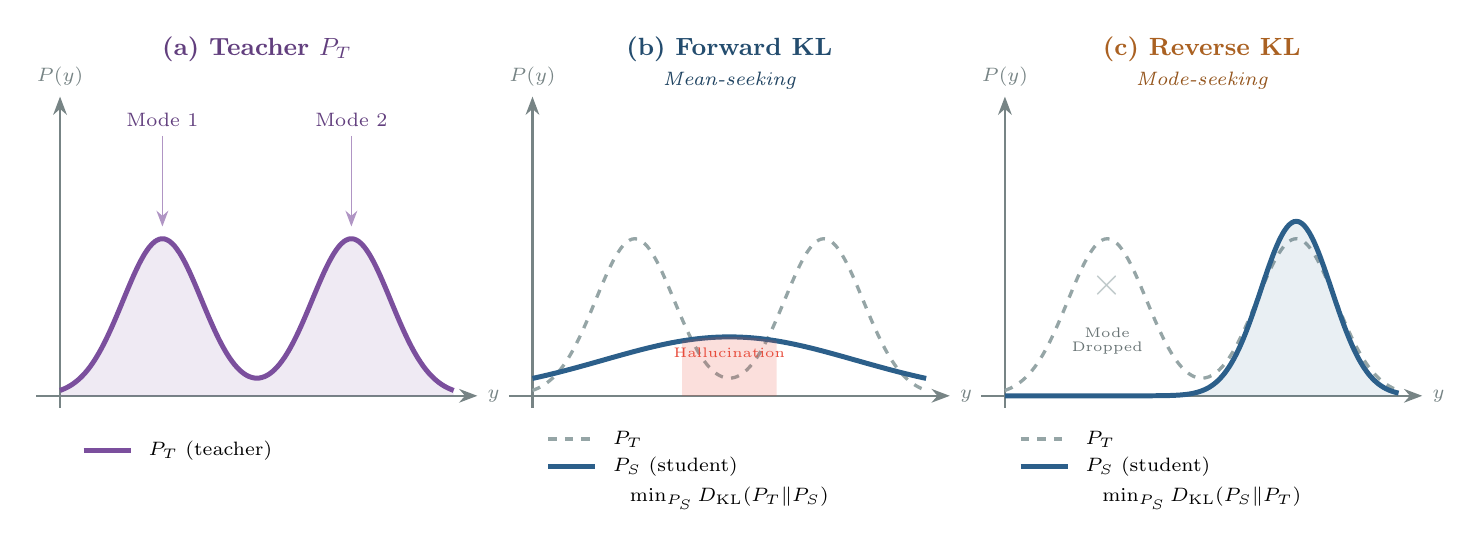
\begin{tikzpicture}[
    >=Stealth,
    annot/.style={font=\scriptsize, #1},
    annot/.default=black,
  ]

  % =================== (a) Teacher Distribution P_T ===================
  \begin{scope}[shift={(0,0)}]
    % Axes
    \draw[->, line width=0.8pt, acadgray!80!black] (-0.3, 0) -- (5.3, 0) 
      node[right, font=\scriptsize] {$y$};
    \draw[->, line width=0.8pt, acadgray!80!black] (0, -0.15) -- (0, 3.8) 
      node[above, font=\scriptsize] {$P(y)$};
    
    % Teacher distribution: bimodal (mu1=1.3, sigma=0.5; mu2=3.7, sigma=0.5)
    \draw[acadpurple, line width=1.8pt, smooth, samples=80, domain=0:5]
      plot (\x, {2.5*(exp(-((\x-1.3)^2)/(2*0.5^2)) + exp(-((\x-3.7)^2)/(2*0.5^2)))/(0.5*sqrt(2*pi))});
    
    % Fill under curve
    \fill[acadpurple, opacity=0.12, smooth, samples=80, domain=0:5]
      plot (\x, {2.5*(exp(-((\x-1.3)^2)/(2*0.5^2)) + exp(-((\x-3.7)^2)/(2*0.5^2)))/(0.5*sqrt(2*pi))})
      -- (5,0) -- (0,0) -- cycle;
    
    % Mode labels
    \node[font=\scriptsize, acadpurple!80!black] at (1.3, 3.5) {Mode 1};
    \node[font=\scriptsize, acadpurple!80!black] at (3.7, 3.5) {Mode 2};
    
    % Arrows to peaks
    \draw[->, acadpurple!60, line width=0.6pt] (1.3, 3.3) -- (1.3, 2.15);
    \draw[->, acadpurple!60, line width=0.6pt] (3.7, 3.3) -- (3.7, 2.15);
    
    % Legend
    \draw[acadpurple, line width=1.8pt] (0.3, -0.7) -- (0.9, -0.7);
    \node[font=\scriptsize, anchor=west] at (1.0, -0.7) {$P_T$ (teacher)};
    
    % Subtitle
    \node[font=\small\bfseries, acadpurple!80!black] at (2.5, 4.4) {(a) Teacher $P_T$};
  \end{scope}

  % =================== (b) Forward KL (Mean-seeking) ===================
  \begin{scope}[shift={(6.0,0)}]
    % Axes
    \draw[->, line width=0.8pt, acadgray!80!black] (-0.3, 0) -- (5.3, 0) 
      node[right, font=\scriptsize] {$y$};
    \draw[->, line width=0.8pt, acadgray!80!black] (0, -0.15) -- (0, 3.8) 
      node[above, font=\scriptsize] {$P(y)$};
    
    % Teacher distribution (gray dashed)
    \draw[acadgray, line width=1.2pt, dashed, smooth, samples=80, domain=0:5]
      plot (\x, {2.5*(exp(-((\x-1.3)^2)/(2*0.5^2)) + exp(-((\x-3.7)^2)/(2*0.5^2)))/(0.5*sqrt(2*pi))});
    
    % Student distribution: wide single peak (mu=2.5, sigma=1.6)
    \draw[acadblue, line width=1.8pt, smooth, samples=80, domain=0:5]
      plot (\x, {3.0*exp(-((\x-2.5)^2)/(2*1.6^2))/(1.6*sqrt(2*pi))});
    
    % Hallucination zone fill (between modes, where student has mass but teacher doesn't)
    \fill[acadred, opacity=0.18, smooth, samples=60, domain=1.9:3.1]
      plot (\x, {3.0*exp(-((\x-2.5)^2)/(2*1.6^2))/(1.6*sqrt(2*pi))})
      -- (3.1, 0) -- (1.9, 0) -- cycle;
    
    % Hallucination label
    \node[font=\tiny, acadred, rotate=0] at (2.5, 0.55) {Hallucination};
    
    % Legend
    \draw[acadgray, line width=1.2pt, dashed] (0.2, -0.55) -- (0.8, -0.55);
    \node[font=\scriptsize, anchor=west] at (0.9, -0.55) {$P_T$};
    \draw[acadblue, line width=1.8pt] (0.2, -0.9) -- (0.8, -0.9);
    \node[font=\scriptsize, anchor=west] at (0.9, -0.9) {$P_S$ (student)};
    
    % Subtitle
    \node[font=\small\bfseries, acadblue!80!black] at (2.5, 4.4) {(b) Forward KL};
    \node[font=\scriptsize\itshape, acadblue!70!black] at (2.5, 4.0) {Mean-seeking};
    
    % Formula
    \node[font=\scriptsize, anchor=center] at (2.5, -1.3) 
      {$\min_{P_S} D_{\mathrm{KL}}(P_T \| P_S)$};
  \end{scope}

  % =================== (c) Reverse KL (Mode-seeking) ===================
  \begin{scope}[shift={(12.0,0)}]
    % Axes
    \draw[->, line width=0.8pt, acadgray!80!black] (-0.3, 0) -- (5.3, 0) 
      node[right, font=\scriptsize] {$y$};
    \draw[->, line width=0.8pt, acadgray!80!black] (0, -0.15) -- (0, 3.8) 
      node[above, font=\scriptsize] {$P(y)$};
    
    % Teacher distribution (gray dashed)
    \draw[acadgray, line width=1.2pt, dashed, smooth, samples=80, domain=0:5]
      plot (\x, {2.5*(exp(-((\x-1.3)^2)/(2*0.5^2)) + exp(-((\x-3.7)^2)/(2*0.5^2)))/(0.5*sqrt(2*pi))});
    
    % Student distribution: narrow peak at mode 2 (mu=3.7, sigma=0.45)
    \draw[acadblue, line width=1.8pt, smooth, samples=80, domain=0:5]
      plot (\x, {2.5*exp(-((\x-3.7)^2)/(2*0.45^2))/(0.45*sqrt(2*pi))});
    
    % Fill student
    \fill[acadblue, opacity=0.1, smooth, samples=80, domain=0:5]
      plot (\x, {2.5*exp(-((\x-3.7)^2)/(2*0.45^2))/(0.45*sqrt(2*pi))})
      -- (5,0) -- (0,0) -- cycle;
    
    % Mode dropped marker at Mode 1
    \node[font=\Large, acadgray!60] at (1.3, 1.4) {$\times$};
    \node[font=\tiny, acadgray!70!black, text width=1.2cm, align=center] at (1.3, 0.7) {Mode\\[-1pt]Dropped};
    
    % Legend
    \draw[acadgray, line width=1.2pt, dashed] (0.2, -0.55) -- (0.8, -0.55);
    \node[font=\scriptsize, anchor=west] at (0.9, -0.55) {$P_T$};
    \draw[acadblue, line width=1.8pt] (0.2, -0.9) -- (0.8, -0.9);
    \node[font=\scriptsize, anchor=west] at (0.9, -0.9) {$P_S$ (student)};
    
    % Subtitle
    \node[font=\small\bfseries, acadorange!80!black] at (2.5, 4.4) {(c) Reverse KL};
    \node[font=\scriptsize\itshape, acadorange!70!black] at (2.5, 4.0) {Mode-seeking};
    
    % Formula
    \node[font=\scriptsize, anchor=center] at (2.5, -1.3) 
      {$\min_{P_S} D_{\mathrm{KL}}(P_S \| P_T)$};
  \end{scope}

\end{tikzpicture}
\end{document}
